% !TEX root = ../Oliveras_Talk.tex
\section{Asymptotic Models}



% ==============================================================================================
\begin{frame}[t]\frametitle{Nondimensionalization}
    We introduce the nondimensional quantities as follows:
    \begin{eqnarray*}
        &\displaystyle x = x^*L, \quad z = z^* h, \quad t = \frac{L}{c_0}t^*, \quad c_0 = \sqrt{gh},\quad \emA{\epsilon = \frac{a}{h}}, \quad \emA{\mu = \frac{h}{L}},\\&\\
        &\displaystyle \eta = a\eta^*,\qquad \frac{p(x,-h,t)-\rho g h}{\rho} = \epsilon P_d^*,\qquad Q = \frac{Lga}{c_0}Q^*,\qquad q = \frac{Lga}{c_0}q^*,
    \end{eqnarray*}
    \vfill
    \pause
    This yields the \emA{\bf nondimensional relationship}
        \[\bint{ P_d\,\varphi_{zz}} = \sint{\eta\varphi_{zz} + \mu^2\eta_{tt}\varphi_z + \epsilon\mu^2\left(\eta_t^2\varphi_{zz} + \left(\eta\eta_x + 2\left(q_t\eta_x - q_x\eta_t\right)\right)\varphi_{xz}\right)},\]
    where \(\varphi\) solves \(\mu^2\varphi_{xx} + \varphi_{zz} = 0\).  
\end{frame}
% ==============================================================================================


% ==============================================================================================
\begin{frame}[t]\frametitle{What effect does \(\varphi\) have?}
    A logical question is \emA{\bf what effect does the choice of \(\varphi\) have?}    
    
    \[\bint{ P_d\,\varphi_{zz}} = \sint{\eta\varphi_{zz} + \mu^2\eta_{tt}\varphi_z + \epsilon\mu^2\left(\eta_t^2\varphi_{zz} + \left(\eta\eta_x + 2\left(q_t\eta_x - q_x\eta_t\right)\right)\varphi_{xz}\right)},\]
    \pause
    \vspace*{.5in}
    \only<2>{
        \begin{block}{Remark \#1}
            Choosing \emC{{\(\varphi = e^{-ikx}\sinh(\mu k (z + 1))\)}} clearly eliminates the relationship between the pressure at the bottom.  This equation combined with either (A) or (B) \emph{completes} the system in the surface variables \(\eta\) and \(q\).
        \end{block}
    }
    \only<3>{
        \begin{block}{Remark \#2}
            We have seen the impact of the choice of \emC{\(\varphi\)} in our previous work - specifically, different choices of \(\varphi\) resulted in more numerically stable algorithms to create pressure contours in the presence of constant vorticity.
        \end{block}
    }
\end{frame}
% ==============================================================================================

% ==============================================================================================
\begin{frame}\frametitle{What effect does \(\varphi\) have?}
\begin{center}
    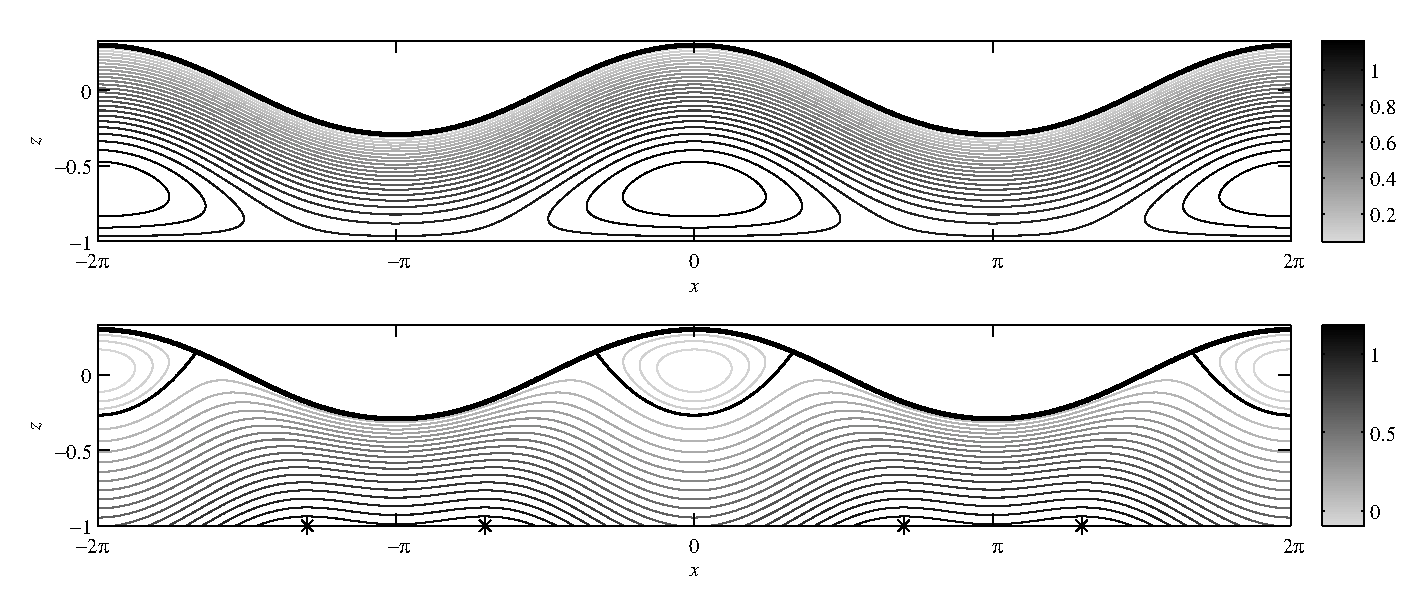
\includegraphics[width=.9\textwidth]{images/const_vorticity_pressure_streamline_contour_gamma_3.eps}
\end{center}
\end{frame}
% ==============================================================================================



% ==============================================================================================
\begin{frame}[t]\frametitle{What effect does \(\varphi\) have?}
    A logical question is \emA{\bf what effect does the choice of \(\varphi\) have?}    
    
    \[\bint{ P_d\,\varphi_{zz}} = \sint{\eta\varphi_{zz} + \mu^2\eta_{tt}\varphi_z + \epsilon\mu^2\left(\eta_t^2\varphi_{zz} + \left(\eta\eta_x + 2\left(q_t\eta_x - q_x\eta_t\right)\right)\varphi_{xz}\right)},\]
    \vspace*{.5in}
    \begin{block}{\Large{Goal}}
            ~\\Can we exploit a variety of choices for \(\varphi\) to eliminate the spatial dependence in order to create a direct \emC{\bf time-series} map?\\~\\
        \end{block}
\end{frame}
% ==============================================================================================

% ==============================================================================================
\begin{frame}[t]\frametitle{Pressure - choosing \(\varphi =e^{-ikx}\cosh(\mu k(z+1))\)}
    \emA{\bf Choosing \(\varphi = e^{-ikx}\cosh(\mu k(z+1))\):}

    \[\displaystyle\fint{\left(\eta+\epsilon\mu^2\eta_t^2\right)\mathcal{C} + \left(\frac{\mu}{k}\eta_{tt}-i\epsilon\mu\left(\eta\eta_x + 2\left(q_t\eta_x-q_x\eta_t\right)\right)\right)\mathcal{S}}=\fint{P_d},\] 
    ~\\
    where \(P_d = (p(x,-h,t)-\rho g h)/\rho\), \(\mathcal{S} = \sinh(\mu k (\epsilon\eta+1))\), and \(\mathcal{C} = \cosh(\mu k (\epsilon\eta+1))\).
    \vfill

    \pause
    \emA{\bf Taking the balance \(\epsilon\sim\mu^2\):}
        \[\hat{P}_{d} =\hat{\eta}+ \epsilon\hat{\eta}_{tt} + \frac{\epsilon k^2}{2}\hat{\eta} + \mathcal{O}(\epsilon^2)\]
    \pause
    It is worth noting that at leading order, we recover precisely the \emA{\bf hydrostatic approximation}.  \pause \emC{\bf Can we do more?}
\end{frame}
% ==============================================================================================


% ==============================================================================================
\begin{frame}[t]
	\frametitle{Comparison of various asymptotic formulae with \(\epsilon \sim\mu^2\).}
	\vfill
    \begin{table}[htp]
        \centering
        {\begin{tabular}{p{.25\textwidth}p{.05\textwidth}p{.54\textwidth}r>{\raggedleft}p{.1\textwidth}}\toprule
            Choice of \(\varphi\) && Resulting Model &\\
            \hline
            \(\displaystyle \varphi = e^{-ikx}\cosh(\mu k (z + 1))\) && \(\displaystyle P_d = \eta + \epsilon\left(\eta_{tt} -\frac{1}{2}\eta_{xx}\right) + \mathcal{O}(\epsilon^2)\)&\\
            &&&\\ &&&\\
            \(\displaystyle \varphi = e^{-ikx}\cosh(\mu kz)\) && \(\displaystyle \left(1 - \frac{\epsilon}{2}\partial_x^2\right)P_d = \eta + \mathcal{O}(\epsilon^2)\)&\\ && \\ &&&\\
            \(\displaystyle \varphi = e^{-ikx}\sinh(\mu kz)\) && \(\displaystyle \left(1 - \frac{\epsilon}{6}\partial_x^2\right)P_d = \eta - \left(\frac{1}{2}\eta^2 + \epsilon\left(\partial_x^{-1}\eta_t\right)^2\right) + \mathcal{O}(\epsilon^2)\)&\\\bottomrule
        \end{tabular}}
    \end{table}
\end{frame}

% ==============================================================================================


% ==============================================================================================
\begin{frame}[t]\frametitle{Three equations for two unknowns? }
    The three equations are consistent provided: 
    \[\eta_{tt} - \eta_{xx} = \epsilon\partial_x^2\left[\frac{1}{3}\eta_{xx} + \frac{1}{2}\eta^2 + \left(\partial_x^{-1}\eta_t\right)^2\right] + \mathcal{O}(\epsilon^2).\]
\pause
So, how do we use this in conjunction with the following?
    \begin{itemize}
        \item[] \(\displaystyle P_d = \eta + \epsilon\left(\eta_{tt} -\frac{1}{2}\eta_{xx}\right) + \mathcal{O}(\epsilon^2)\)\\
        \item[] \(\displaystyle \left(1 - \frac{\epsilon}{2}\partial_x^2\right)P_d = \eta + \mathcal{O}(\epsilon^2)\)\\
        \item[] \(\displaystyle \left(1 - \frac{\epsilon}{6}\partial_x^2\right)P_d = \eta - \left(\frac{1}{2}\eta^2 + \epsilon\left(\partial_x^{-1}\eta_t\right)^2\right) + \mathcal{O}(\epsilon^2)\)\\
    \end{itemize}
\pause
\vfill

\emC{\bf Back-substitute the following:} \(\eta_{xx} = \eta_{tt} + \mathcal{O}(\epsilon) \qquad \text{and}\qquad P_d = \eta + \mathcal{O}(\epsilon)\)

\end{frame}
% ==============================================================================================



% ==============================================================================================
\begin{frame}[t]\frametitle{Final Asymptotic Relationship}
    Thus, we end with:
    \[\eta = P_d - \frac{\epsilon}{2}P_{d,tt} + \mathcal{O}(\epsilon^2) \qquad \qquad \eta = P_d - \frac{h}{g}P_{d,tt} + \ldots\]
    \pause
    \vfill
    This formulation has \emA{\bf completely eliminated the spatial component}.  \\~\\ \pause
    
    We have a \emA{\bf direct map} from \(P_d(x_i,t_j) \to \eta(x_i,t_j)\) provided that we have a method to approximate \(P_{d,tt}(x_i,t_j)\)\\~\\ \pause
    
    Despite being accurate to $\mathcal{O}(\epsilon^2)$, the equation remains \emA{\bf linear}. \pause
    \vfill

    Of course, we don't expect that it will perform as well as the fully nonlinear model, but let's see what happens.
\end{frame}
% ==============================================================================================
